\section{神经网络}

\subsection{神经网络示意图}
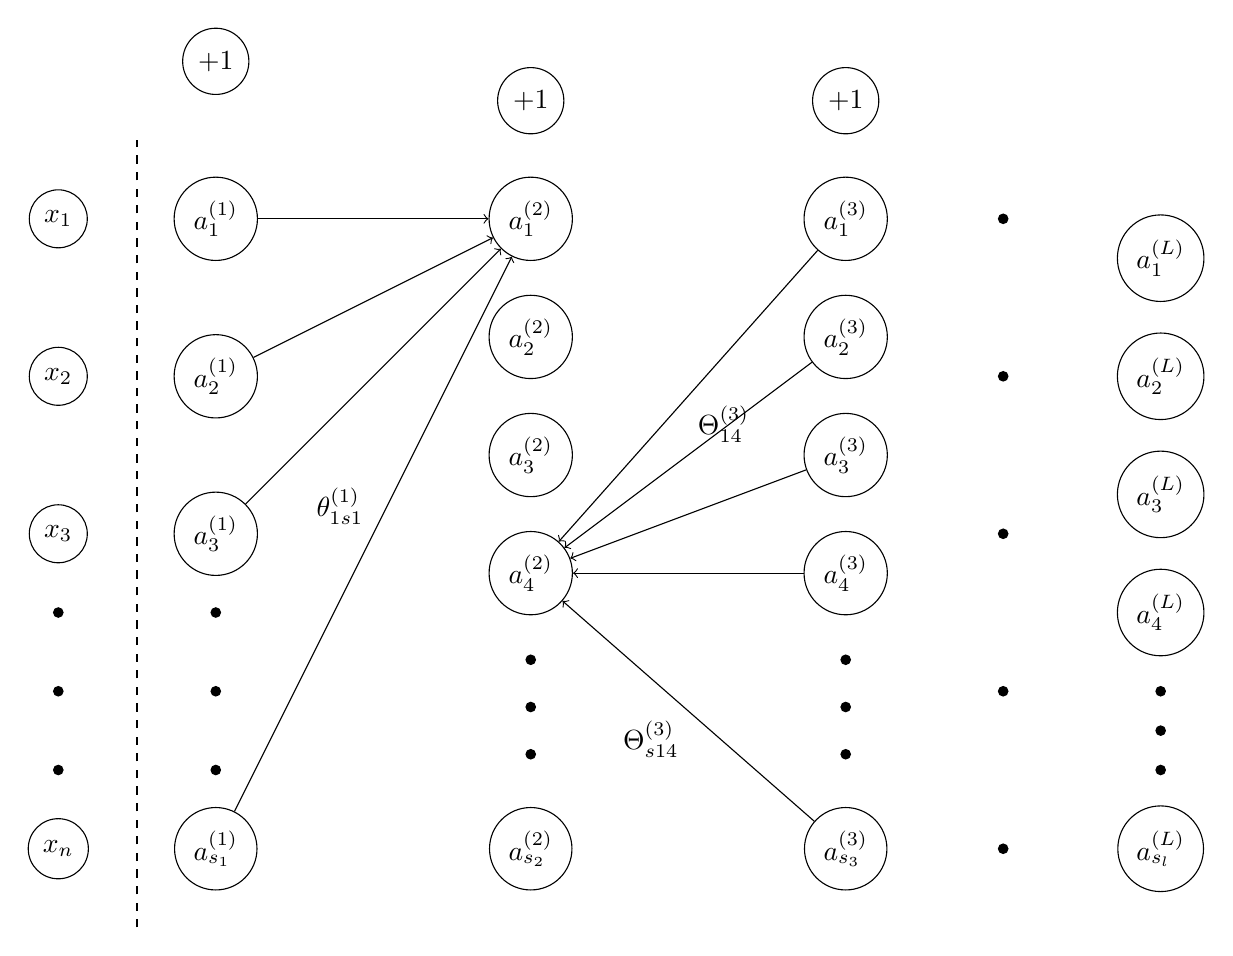
\begin{tikzpicture}
\tikzset{
	a/.style={circle, draw=black}
}

% x
% \node[a] (x_0) at(0,10) {$x_0=+1$};
\node[a] (x_1) at(0,8) {$x_1$};
\node[a] (x_2) at(0,6) {$x_2$};
\node[a] (x_3) at(0,4) {$x_3$};
\filldraw (0,3) circle (.06);
\filldraw (0,2) circle (.06);
\filldraw (0,1) circle (.06);
\node[a] (x_n) at(0,0) {$x_n$};

% X与a的分隔线
\draw [dashed] (1,-1) -- (1,9);

% a^{(1)}
\node[a] (a_10) at(2,10)   {$+1$};
\node[a] (a_11) at(2,8)   {$a_1^{(1)}$};
\node[a] (a_12) at(2,6) {$a_2^{(1)}$};
\node[a] (a_13) at(2,4)   {$a_3^{(1)}$};
\filldraw (2,3) circle (.06);
\filldraw (2,2) circle (.06);
\filldraw (2,1) circle (.06);
\node[a] (a_1s1) at(2,0) {$a_{s_1}^{(1)}$};

% a^{(2)}
\node[a] (a_20) at(6,9.5) {$+1$};
\node[a] (a_21) at(6,8.0) {$a_1^{(2)}$};
\node[a] (a_22) at(6,6.5) {$a_2^{(2)}$};
\node[a] (a_23) at(6,5.0) {$a_3^{(2)}$};
\node[a] (a_24) at(6,3.5) {$a_4^{(2)}$};
\filldraw (6,2.4) circle (.06);
\filldraw (6,1.8) circle (.06);
\filldraw (6,1.2) circle (.06);
\node[a] (a_2s2) at(6,0) {$a_{s_2}^{(2)}$};

% a^{(3)}
\node[a] (a_30) at(10,9.5) {$+1$};
\node[a] (a_31) at(10,8.0) {$a_1^{(3)}$};
\node[a] (a_32) at(10,6.5) {$a_2^{(3)}$};
\node[a] (a_33) at(10,5.0) {$a_3^{(3)}$};
\node[a] (a_34) at(10,3.5) {$a_4^{(3)}$};
\filldraw (10,2.4) circle (.06);
\filldraw (10,1.8) circle (.06);
\filldraw (10,1.2) circle (.06);
\node[a] (a_3s3) at(10,0) {$a_{s_3}^{(3)}$};

% 中间部分
\filldraw (12,0) circle (.06);
\filldraw (12,2) circle (.06);
\filldraw (12,4) circle (.06);
\filldraw (12,6) circle (.06);
\filldraw (12,8) circle (.06);

% a^{(n)}

\node[a] (a_L1) at(14,7.5) {$a_1^{(L)}$};
\node[a] (a_L2) at(14,6)   {$a_2^{(L)}$};
\node[a] (a_L3) at(14,4.5) {$a_3^{(L)}$};
\node[a] (a_L4) at(14,3)   {$a_4^{(L)}$};
\filldraw (14,2.0) circle (.06);
\filldraw (14,1.5) circle (.06);
\filldraw (14,1.0) circle (.06);
\node[a] (a_Lsl) at(14,0) {$a_{s_l}^{(L)}$};


% 前向算法图例--仅连线:a1 -- a_21
% \draw[->] (a_10) -- (a_21);
\draw[->] (a_11) -- (a_21);
\draw[->] (a_12) -- (a_21);
\draw[->] (a_13) -- (a_21);
% \draw[->] (a_1s1) -- (a_21);

% 前向算法图例--有标注:a1 -- a_21

% \path (a_11) edge[->] node[auto] {$\theta_{11}^{(1)}$} (a_21);
% \path (a_12) edge[->] node[auto] {$\theta_{12}^{(1)}$} (a_21);
% \path (a_13) edge[->] node[auto] {$\theta_{13}^{(1)}$} (a_21);
\path (a_1s1) edge[->] node[auto] {$\theta_{1s1}^{(1)}$} (a_21);


% 向后算法--仅连线: a3 -- a24
% \draw[->] (a_31) -- (a_24);
\draw[->] (a_32) -- (a_24);
\draw[->] (a_33) -- (a_24);
\draw[->] (a_34) -- (a_24);
% \draw[->] (a_3s3) -- (a_24);

% 前后算法图例--有标注:a3 -- a24
\path (a_31) edge[->] node[auto] {$\Theta_{14}^{(3)}$} (a_24);
% \path (a_32) edge[->] node[auto] {$\Theta_{24}^{(3)}$} (a_24);
% \path (a_33) edge[->] node[auto] {$\Theta_{34}^{(3)}$} (a_24);
% \path (a_34) edge[->] node[auto] {$\Theta_{44}^{(3)}$} (a_24);
\path (a_3s3) edge[->] node[auto] {$\Theta_{s14}^{(3)}$} (a_24);


% 下方的标志


\end{tikzpicture}
